\section{Quantencomputer Allgemein}
\label{sec:quantencomputer}
Der Unterschied zwischen einem Quantencomputer und einem normalen Computer ist die Verwendung von Quantenbits \cite{quantencomputer_2024} anstelle der üblichen Bits, womit ein Zweistandsystem \cite{zweizustandssystem_nodate} erstellt wird, wobei ein Qubit entweder einer 1 oder einer 0 entspricht und das System aus mindestens zwei Bits besteht. Damit können verschiedene Werte erstellt werden, wie 1;1, 0;1, 0;0, 1;0, wie in normalen Transistoren.

Der Unterschied zu konventionellen Computern ist nun, dass zwei Qubits, solange keine Messungen des gesamten Systems stattfinden, aus einer Superposition aus 1 und 0 bestehen. 
Das heißt, dass alle vier Werte des Zweistandsystems parallel zueinander existieren können und es möglich machen, mehrere Berechnungen gleichzeitig durchzuführen.\cite{What_is_quantum_computing_nodate}
Dies wird ermöglicht durch die Quantenverschränkung, wobei zwei Systeme so eng miteinander verbunden sind, dass Wissen über den ersten Teil des Systems mit einer Wahrscheinlichkeitsverteilung ein Wissen über den zweiten gibt, ohne den zweiten Teil gemessen zu haben.\cite{quantenverschrankung_2024}

Ein Qubit könnte zum Beispiel die Polarisationsrichtung eines Photons sein, welches von zwei orthogonalen Richtungen gemessen wird \cite{What_is_quantum_computing_nodate}. 

Hier zählen die sinusförmigen elektromagnetischen Wellen als rechts- 
oder linkszirkular und werden dementsprechend als 1 oder 0 angelegt (Abbildung \ref{fig:elektromagnetische_welle}) \cite{electromagnetic_2024}.

\begin{figure}[h]
    \centering
    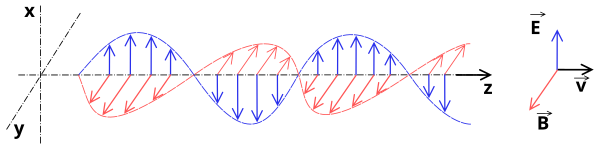
\includegraphics[width=0.45\textwidth]{Onde_electromagnetique.svg.jpg}
    \caption{Eine linear polarisierte elektromagnetische Welle, die in der Z-Achse verläuft.}
    \label{fig:elektromagnetische_welle}
\end{figure}


Andere Implementierungen, ein Zweistandsystem aus Qubits zu erstellen, gibt es auch mit dem Energieniveau von Atomen oder Molekülen bis hin zu Flussrichtungen von Stromkreisen in Supraleitern \cite{supraleitung_nodate}.

Da diese Methoden naturwissenschaftliche Teilchen als Berechnungsbasis nehmen, die von ihrer Größe her kleiner als ein einzelnes Atom sind, spricht man nun von Quantenmechanik. 

Dies führt zu einer der größten Hürden für Quantencomputer, der Dekohärenz, wobei Qubits ihren Quantenzustand durch Umgebungsfaktoren verlieren. Deshalb müssen sie oftmals von außen abgeschirmt und bei Temperaturen nahe dem absoluten Nullpunkt gehalten werden, um den Quantenzustand und somit die Quantenverschränkung aufrechtzuerhalten, die für die Berechnungen nötig sind.

Da die Qubits so sensitiv sind, gibt es auch Schwierigkeiten mit längeren Berechnungen. Oftmals tauchen Fehler in den Qubits auf, die man noch nicht gut genug kompensieren kann. Oft müssen Berechnungen mehrmals durchgeführt werden oder sind in ihrer Länge limitiert.\cite{brubaker_quantum_2024} Es wird weiter an Algorithmen und Systemen geforscht, die sehr vielversprechend sind.

Dies führt zu dem Phänomen "Store now, decrypt later" – jetzt speichern und später entschlüsseln. Zum Beispiel könnten Daten, die mit RSA verschlüsselt werden und heute noch sicher sind, durch die deutlich schnellere Berechnung von Primzahlen durch Quantencomputer in der Zukunft sehr viel leichter entschlüsselt werden. 
Informationen, die heute als sensibel gelten, sind es auch noch in Zukunft, was bedeutet, dass es notwendig ist, heute schon Alternativen für Verschlüsselungen zu verwenden, die gegen leistungsfähigere Quantencomputer gesichert sind.\cite{veritasium_how_2023}

Andere Anwendungsbereiche für Quantencomputer gibt es in der Medizin, 
Materialwissenschaften, Finanzmodellierung 
und Verkehrsoptimierung. \cite{Applications_10_nodate}